\section{Graphs}
This section contains graphical demonstrations of the convergence
properties of FDK. It starts by showing how FDK converges to
a piecewise flat approximation when modelling a line.
It goes on to show the FDK fits generated for some datasets.

\begin{figure}[!htb]
  \minipage{0.3\textwidth}
    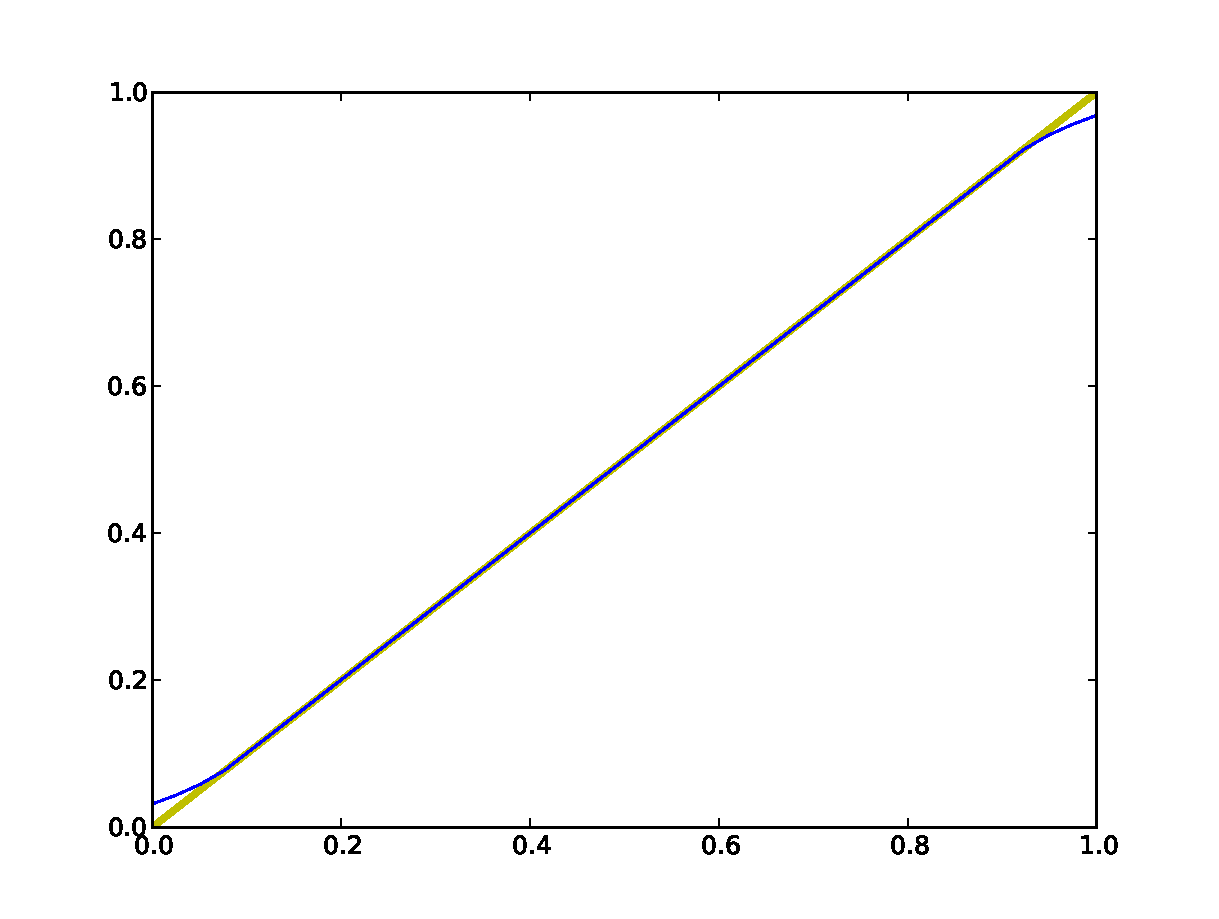
\includegraphics[width=\linewidth]{../writeup/figs/linefit.pdf}
  \endminipage\hfill
  \minipage{0.3\textwidth}
    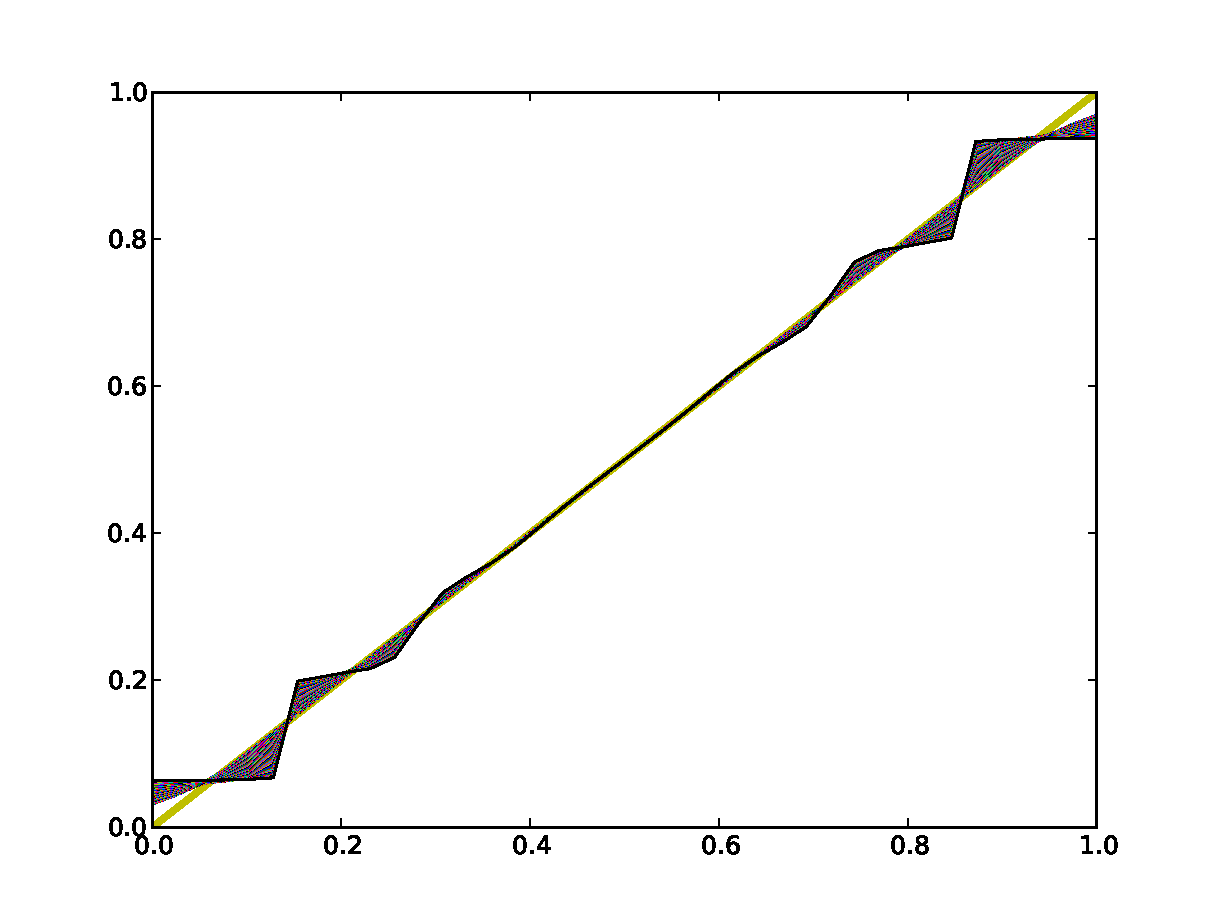
\includegraphics[width=\linewidth]{../writeup/figs/linefitmid.pdf}
  \endminipage\hfill
  \minipage{0.3\textwidth}
    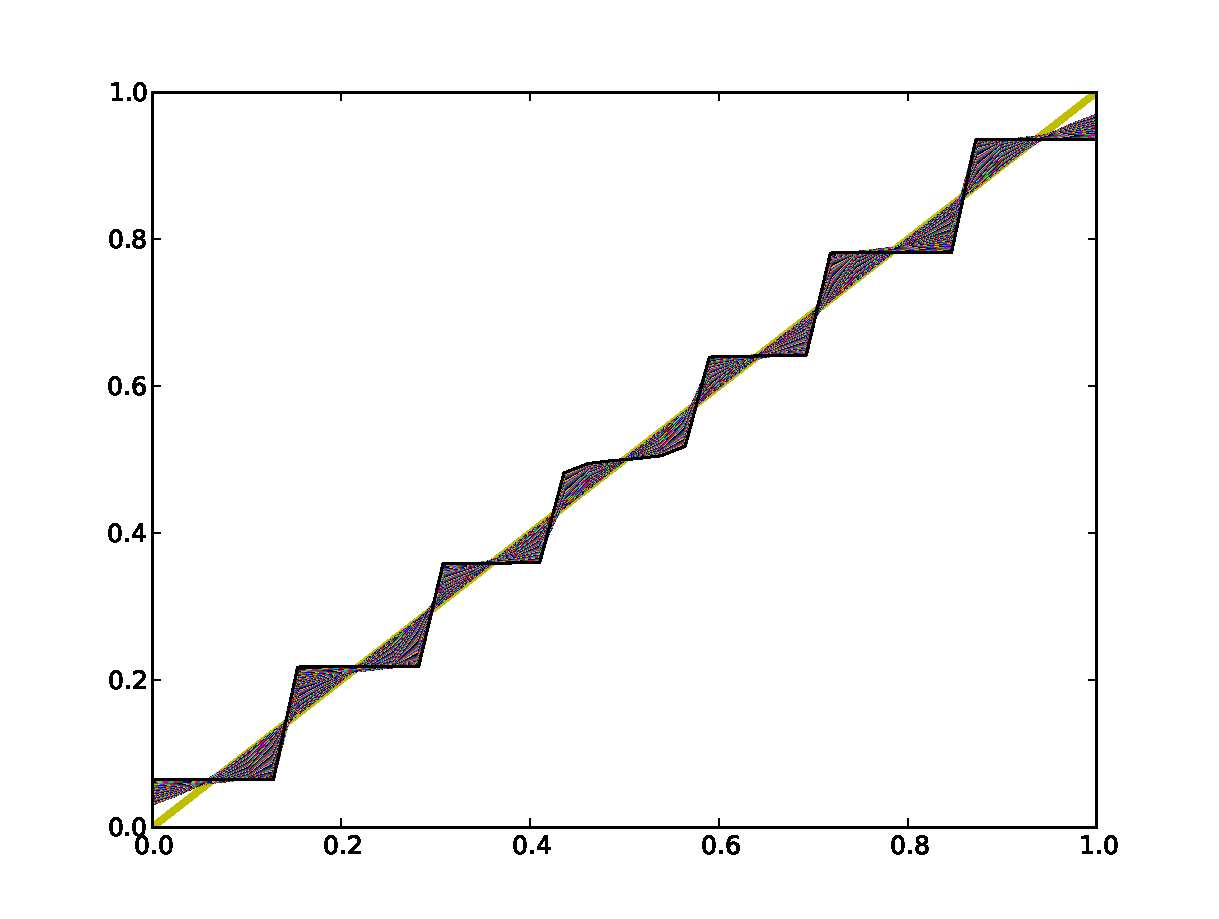
\includegraphics[width=\linewidth]{../writeup/figs/linefitend.pdf}
  \endminipage\hfill
\caption[Fitting a line]{How FDK converges to a piecewise flat approximation
when attempting to fit a line. The figure on the left shows the first fit
$\tilde f_0$ in blue. Note how the fit is biased at the boundaries.
This bias gets amplified over the next several iterations of FDK (middle).
The end result is the piecewise flat approximation on the right.
If we had used a smaller bandwidth there would have been more pieces
in the piecewise flat approximation.}
\end{figure}


When fitting a line, the approximation error increases with every iteration.
For most functions, however, the error goes down for a few iterations before going up.
The following figures show the result fitting some select functions with
different combinations of parameters.

Below we have included plots that show approximation quality of FDK for some
select datasets.
The plots on the left show the dataset (scatter plot), the kernel
regression fit (dotted blue line), the best FDK fit obtained (solid red line), and the
piecewise flat function to which FDK converges for the value of $\alpha$
that produced the best fit (green pluses).
The plots on the right show how the approximation error changes as a function of
iteration number for different values of $\alpha$.
Approximation error is measured as the sum of squared errors, normalized so that the fit produced
by the vanilla kernel regression has unit error. Note how low the error dips and how
few iterations it takes to get there.

\begin{figure}[!htb]
  \minipage{0.46\textwidth}
    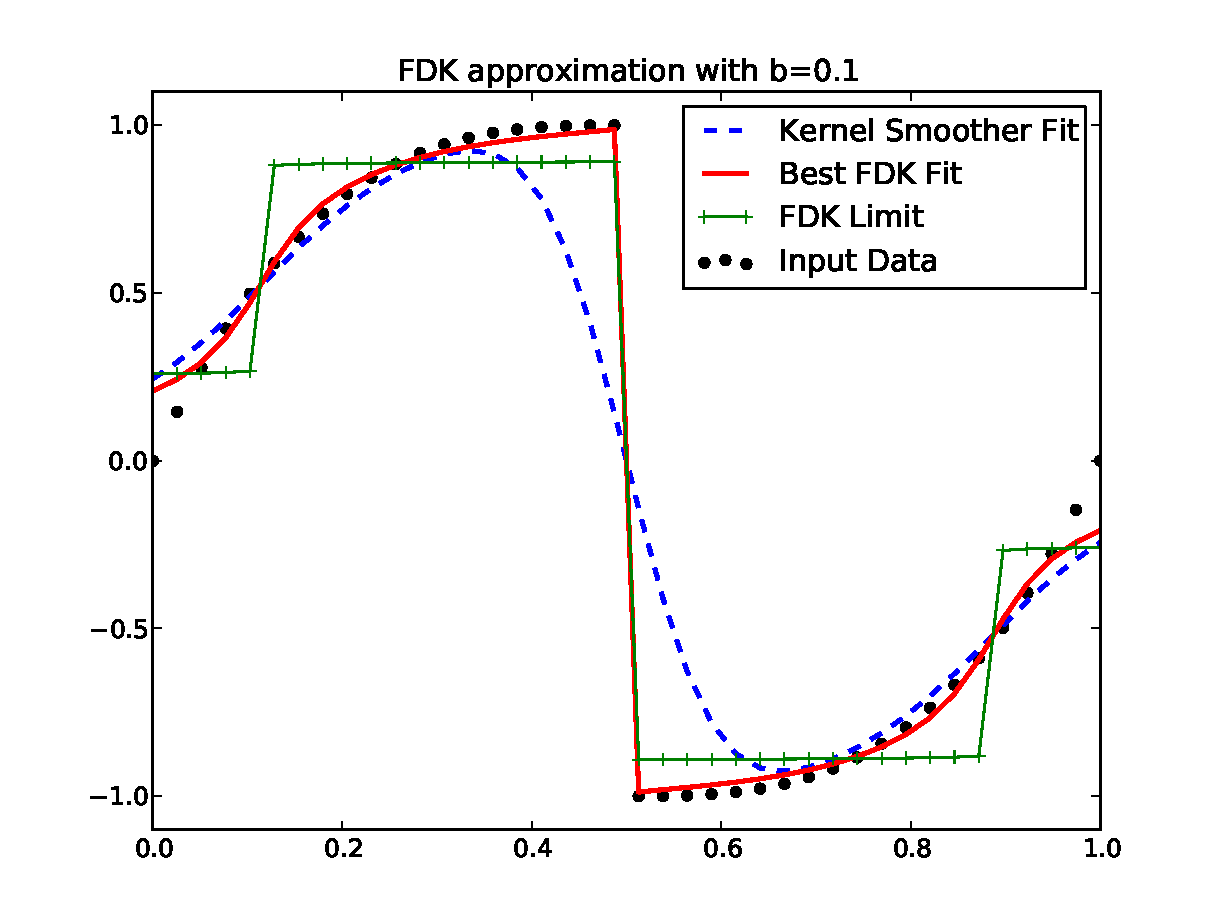
\includegraphics[width=\linewidth]{./figs/flip.pdf}
  \endminipage\hfill
  \minipage{0.46\textwidth}
    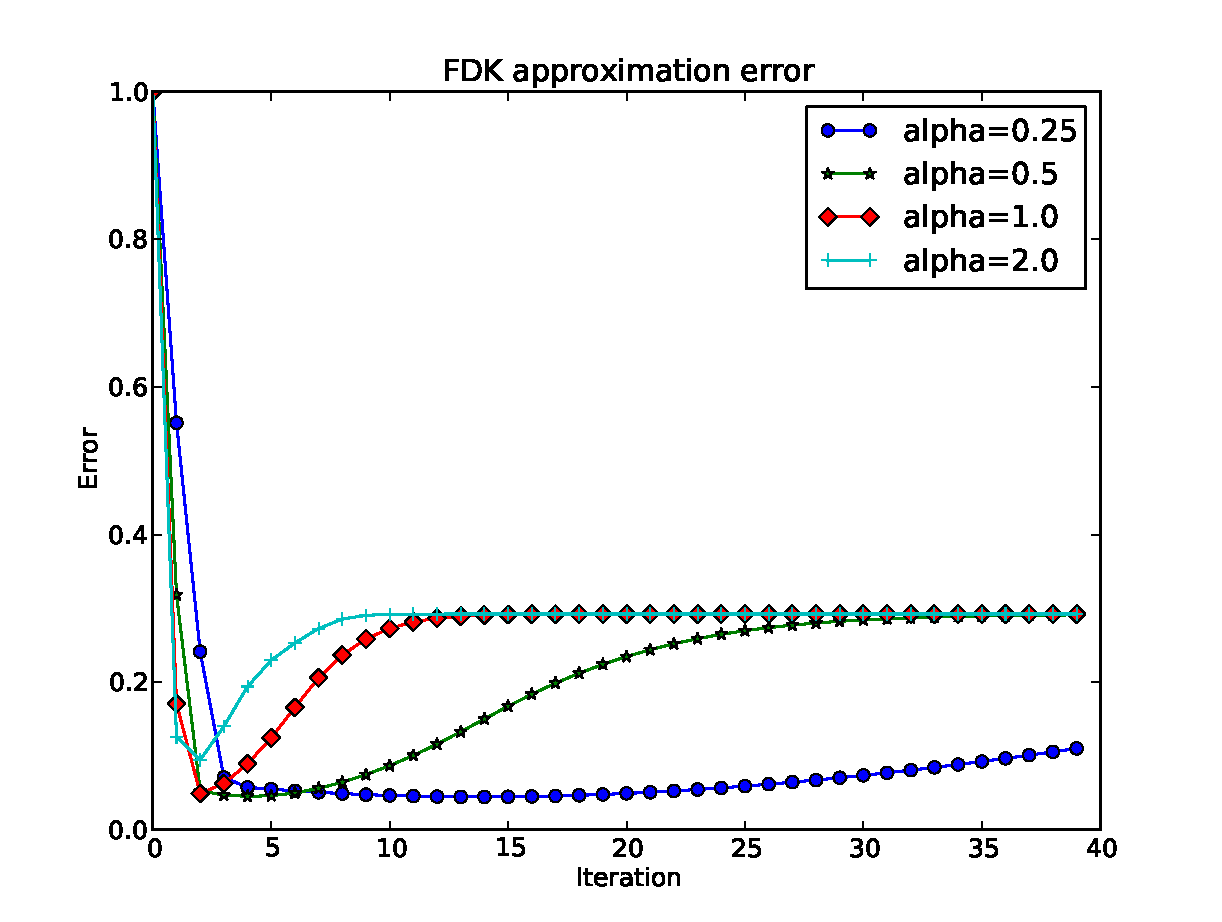
\includegraphics[width=\linewidth]{./figs/fliperr.pdf}
  \endminipage
%\caption[Fitting $x^3 - \mathrm{signum}(x)$]
%{FDK fit for $x^3 - \mathrm{signum}(x)$}
\end{figure}

\begin{figure}[!htb]
  \minipage{0.46\textwidth}
    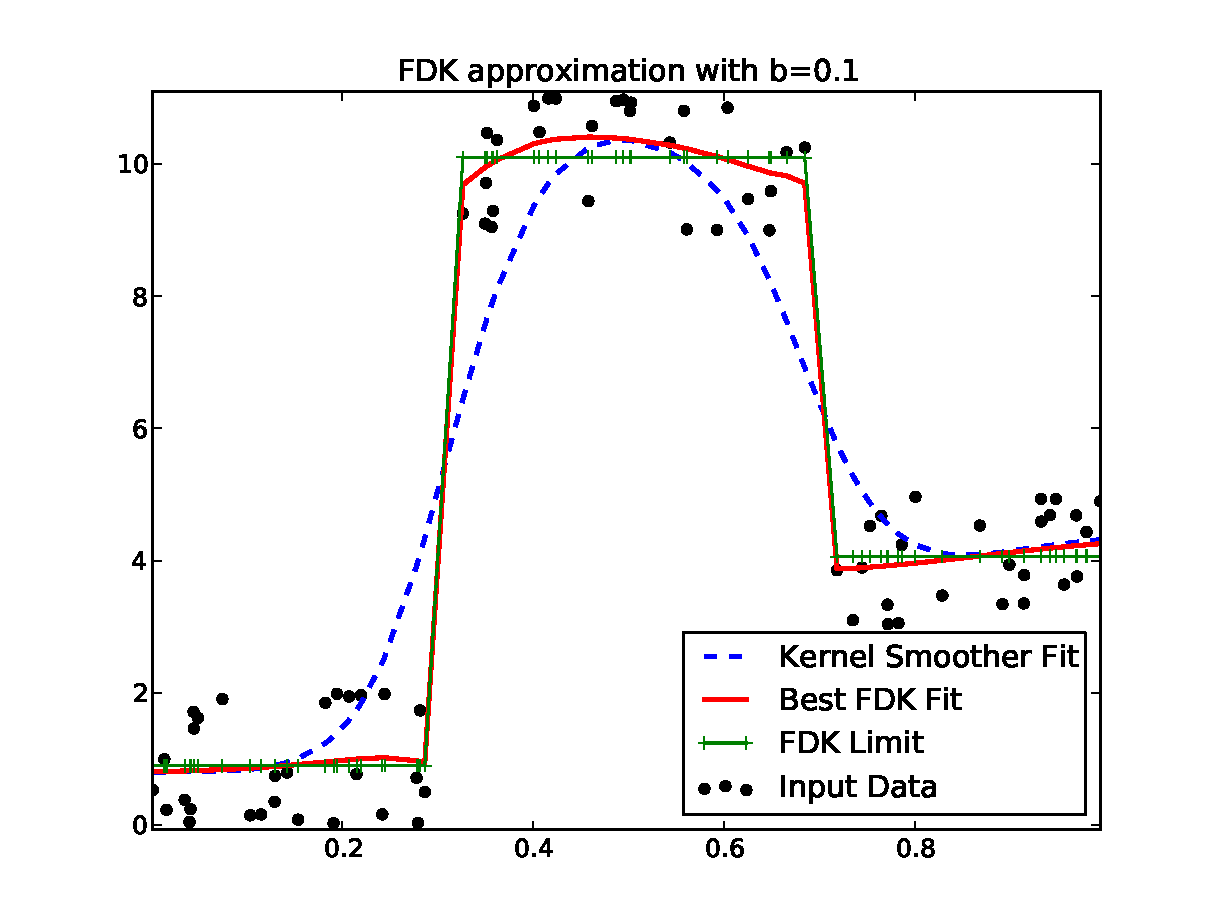
\includegraphics[width=\linewidth]{./figs/3step.pdf}
  \endminipage\hfill
  \minipage{0.46\textwidth}
    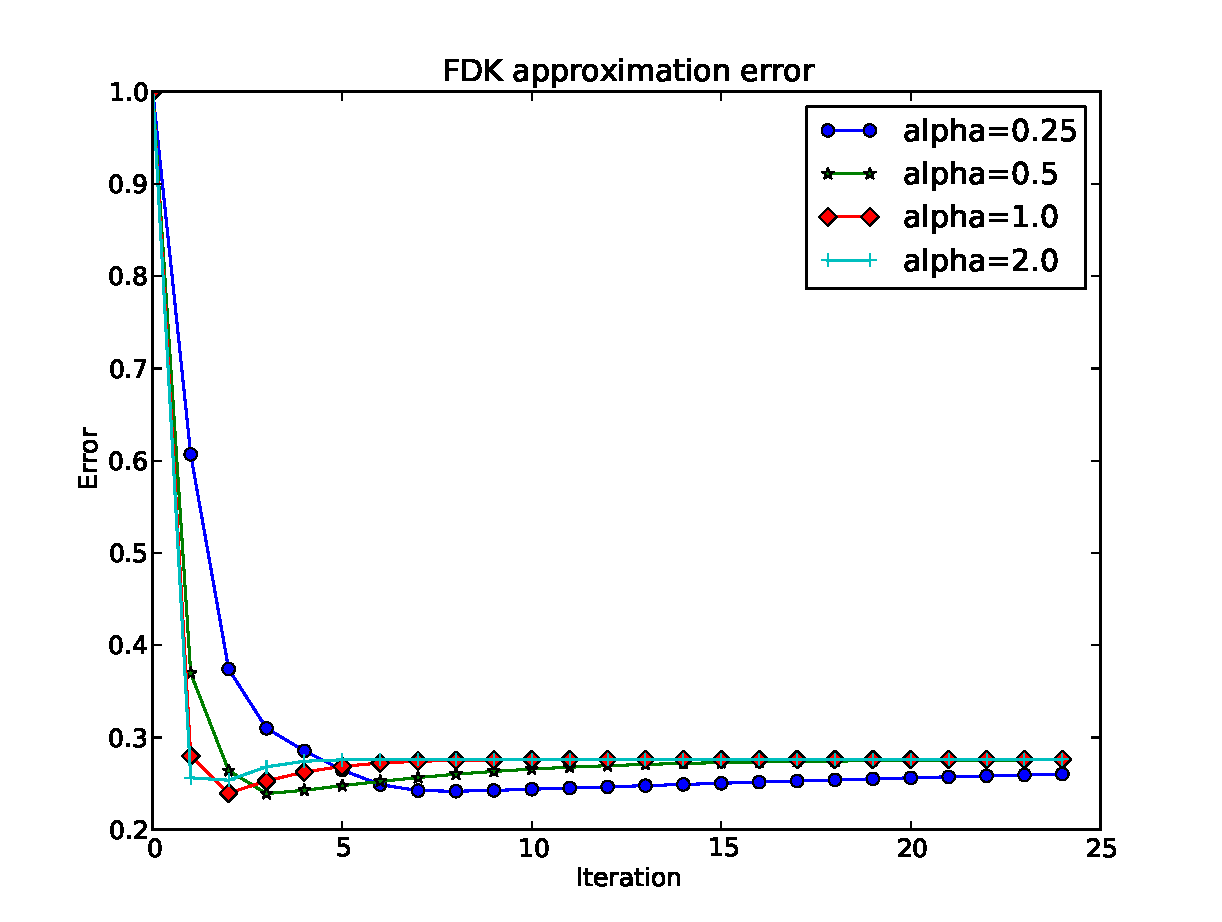
\includegraphics[width=\linewidth]{./figs/3steperr.pdf}
  \endminipage
%\caption[Fitting an order 5 Fourier function with $b = .25$]
%{FDK fit for the Fourier function above, this time with a larger bandwidth.}
\end{figure}

\begin{figure}[!htb]
  \minipage{0.46\textwidth}
    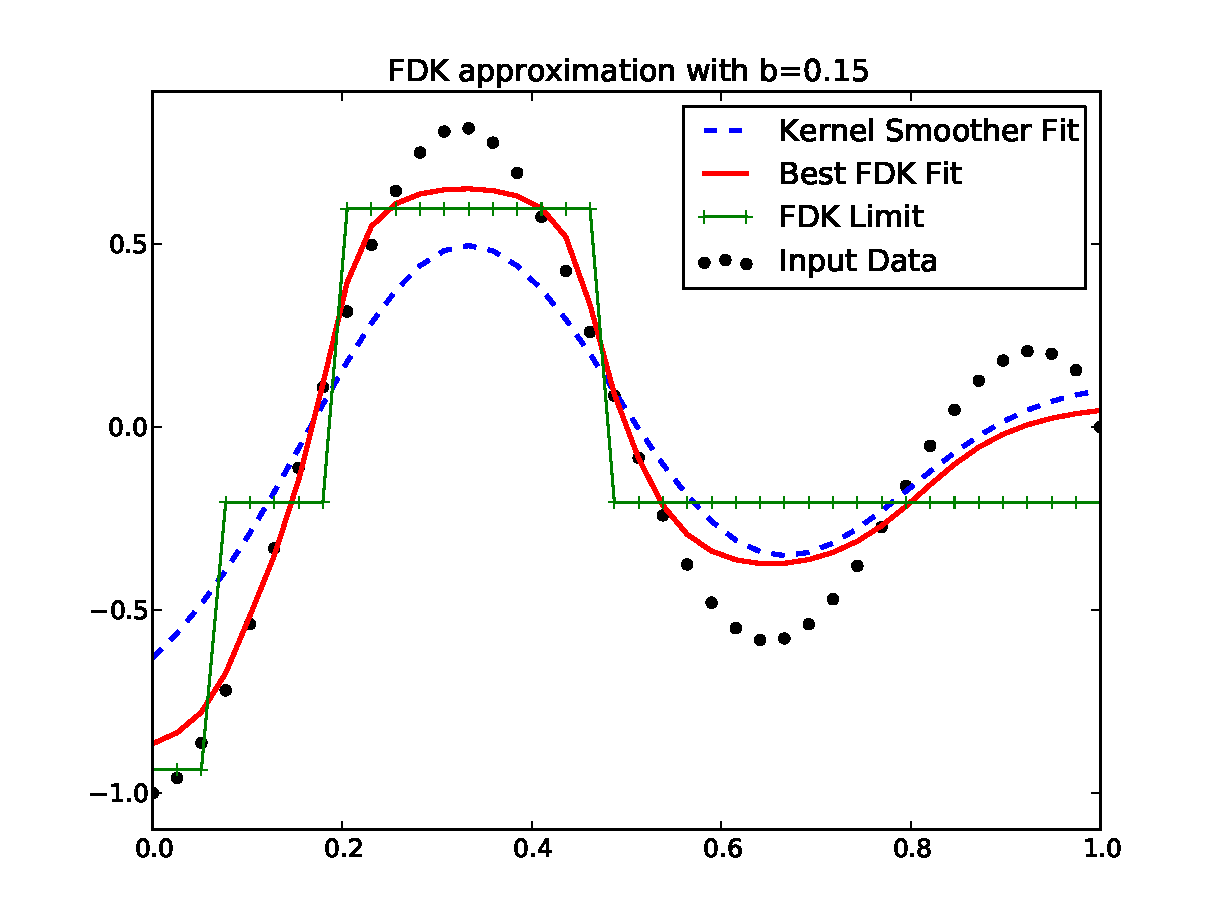
\includegraphics[width=\linewidth]{./figs/sqrtxcosx.pdf}
  \endminipage\hfill
  \minipage{0.46\textwidth}
    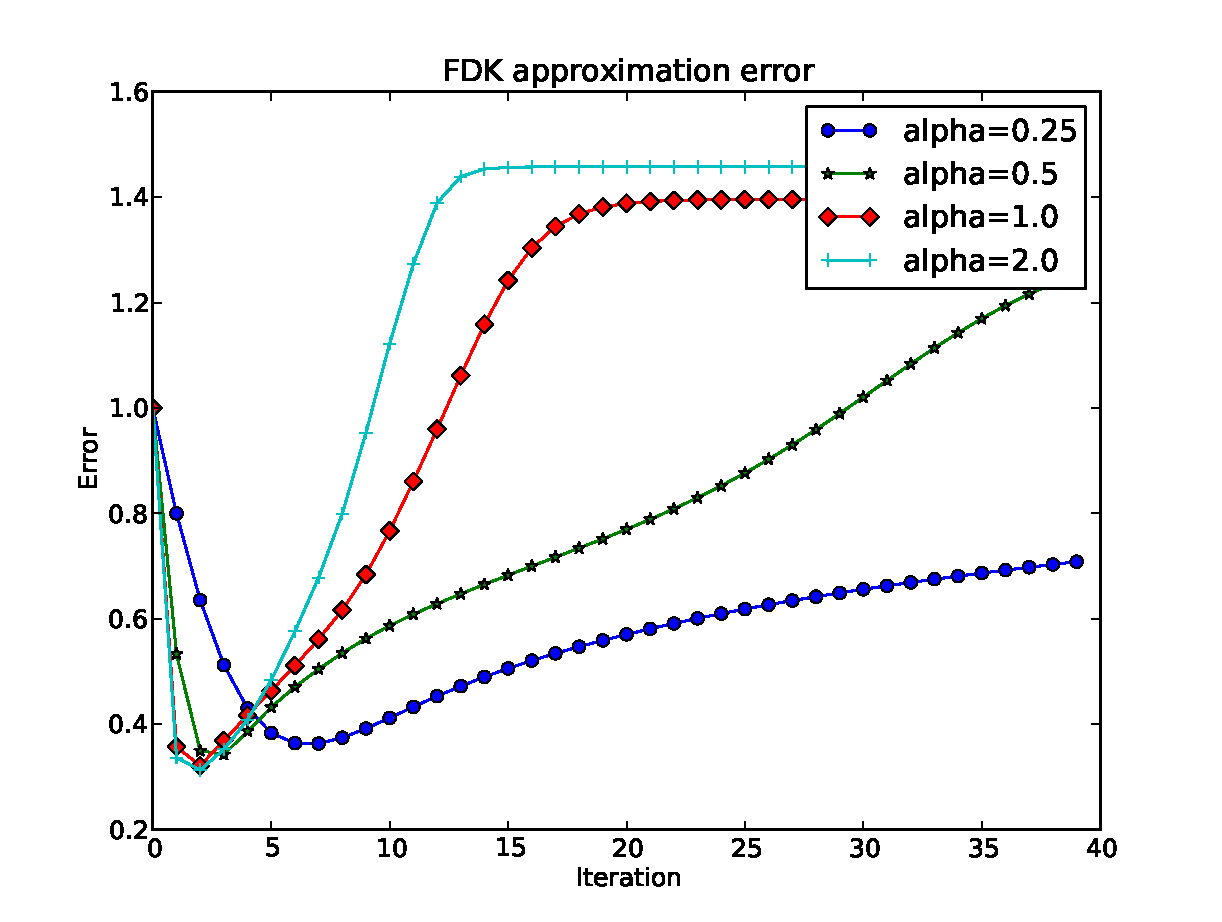
\includegraphics[width=\linewidth]{./figs/sqrtxcosxerr.pdf}
  \endminipage
%\caption[Fitting $-\sqrt{1-x}\cdot\mathrm{cos}(\pi x)$]
%{FDK fit for $-\sqrt{1-x}\cdot\mathrm{cos}(\pi x)$.}
\end{figure}

\begin{figure}[!htb]
  \minipage{0.46\textwidth}
    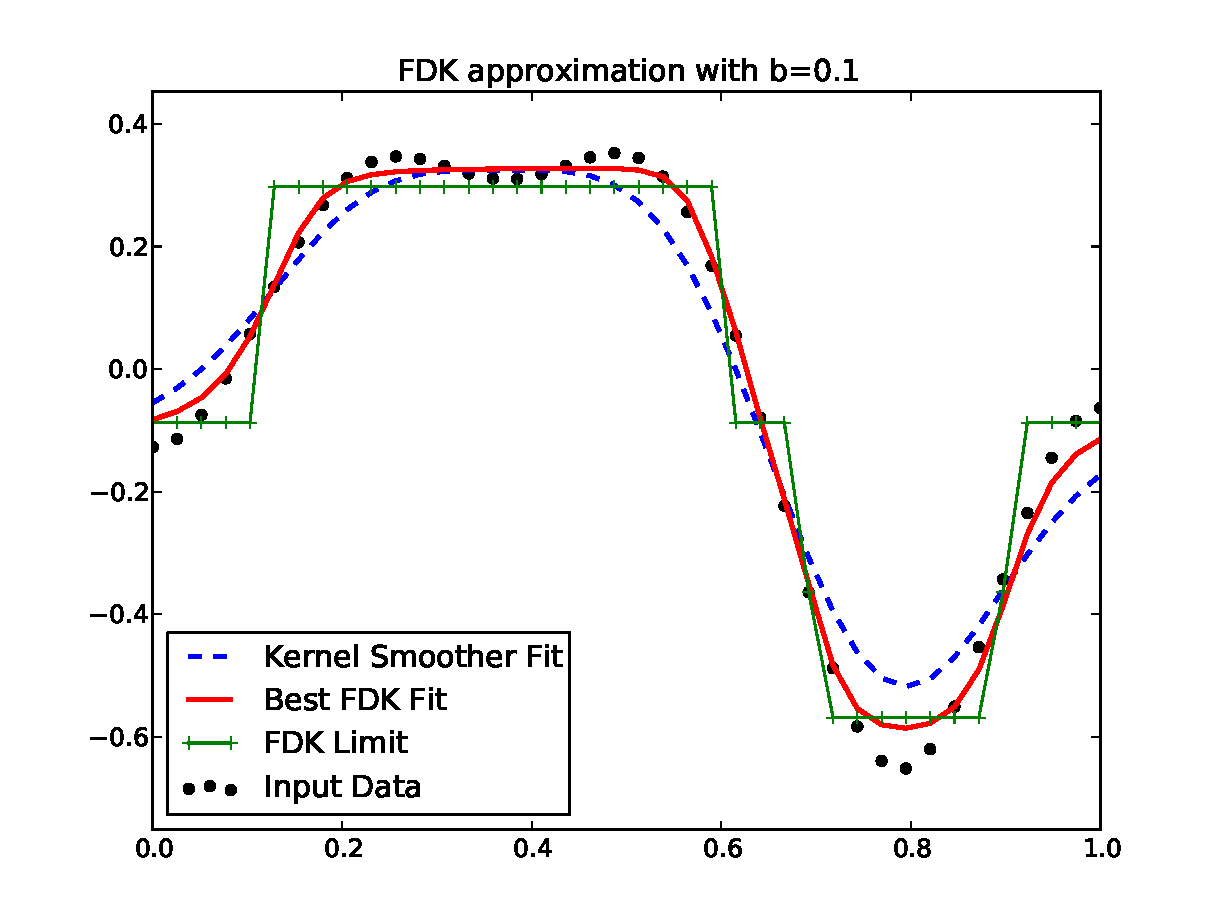
\includegraphics[width=\linewidth]{./figs/bumpy1.pdf}
  \endminipage\hfill
  \minipage{0.46\textwidth}
    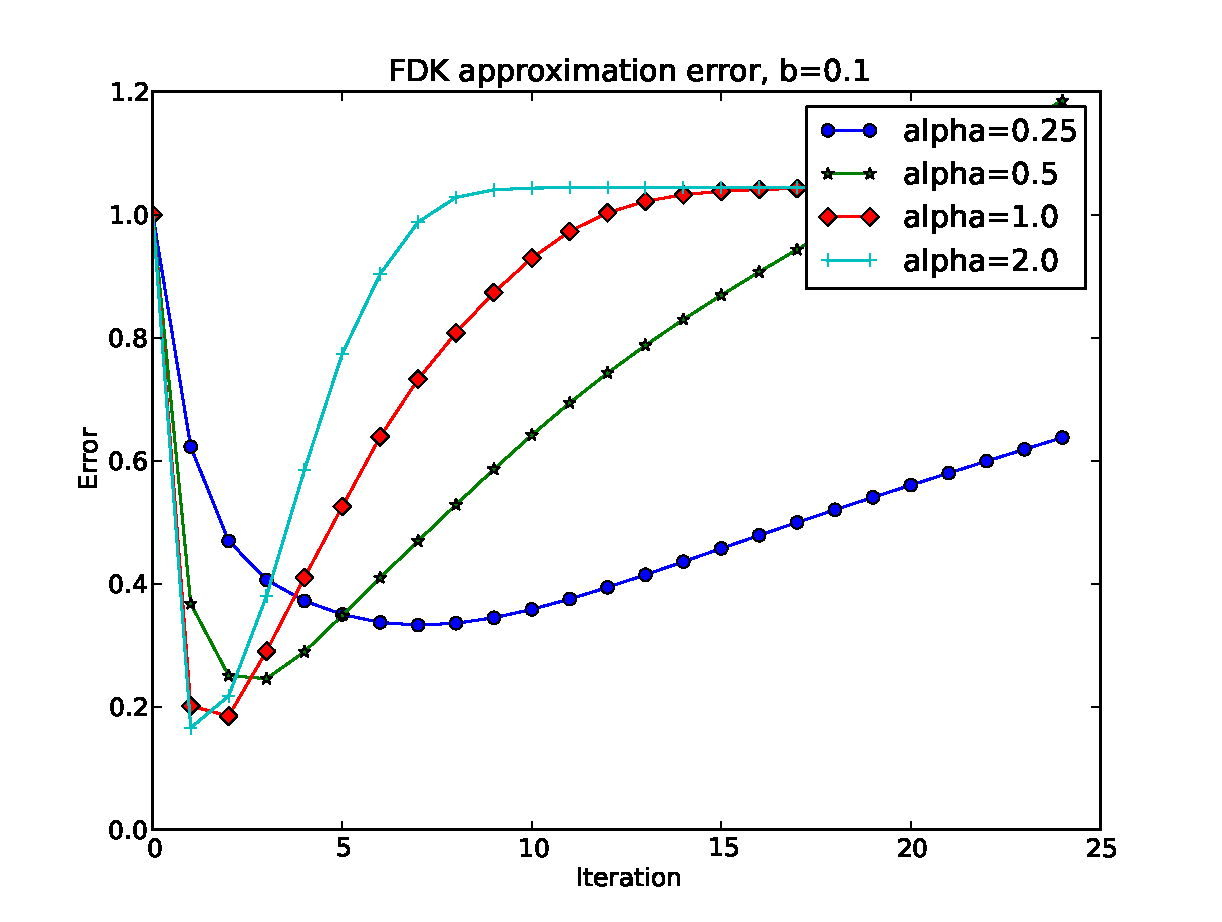
\includegraphics[width=\linewidth]{./figs/bumpyerr1.pdf}
  \endminipage
%\caption[Fitting an order 5 Fourier function with $b = .15$]
%{FDK fit for some order 5 Fourier function.}
\end{figure}

%\begin{figure}[!htb]
%  \minipage{0.12\textwidth}
%    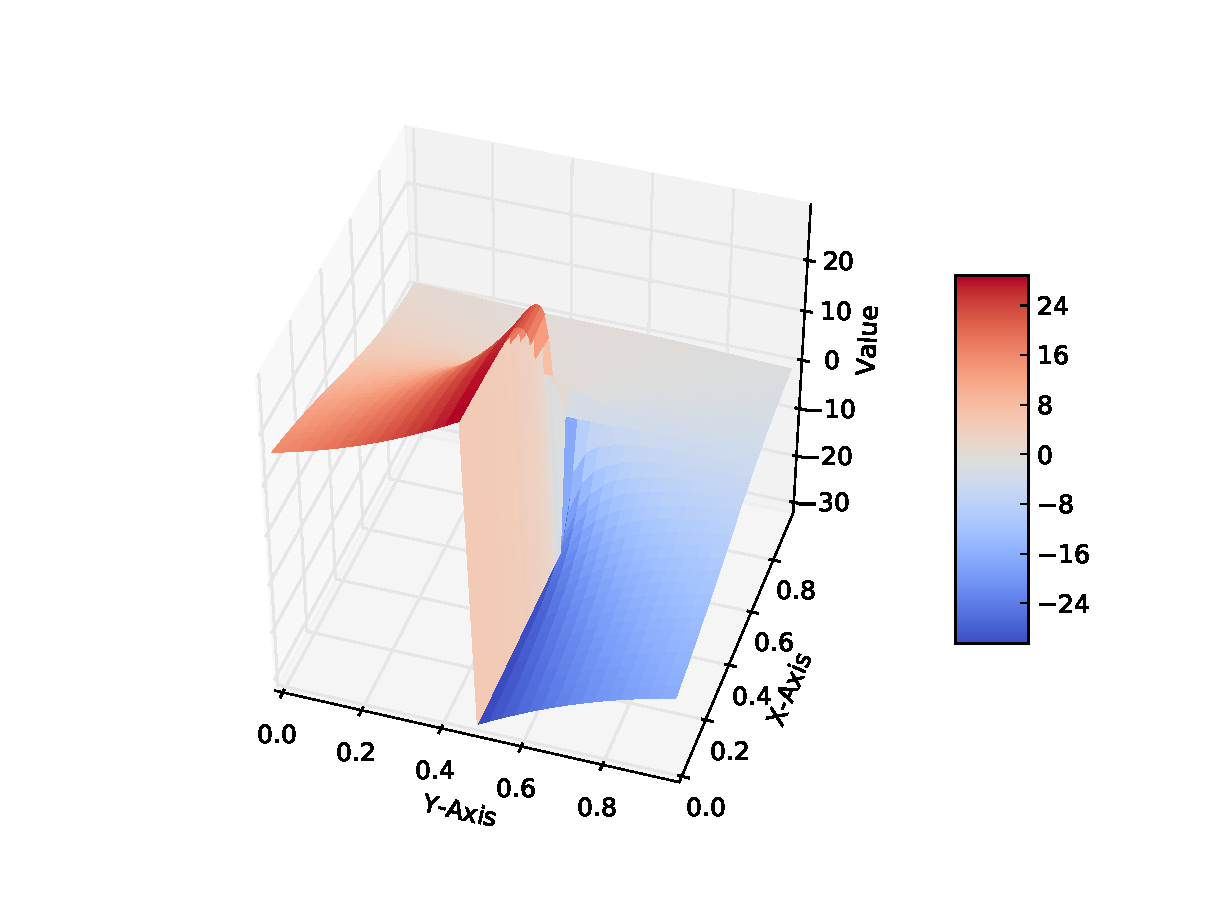
\includegraphics[width=\linewidth]{../writeup/figs/chap4/atan.pdf}
%  \endminipage\hfill
%  \minipage{0.12\textwidth}
%    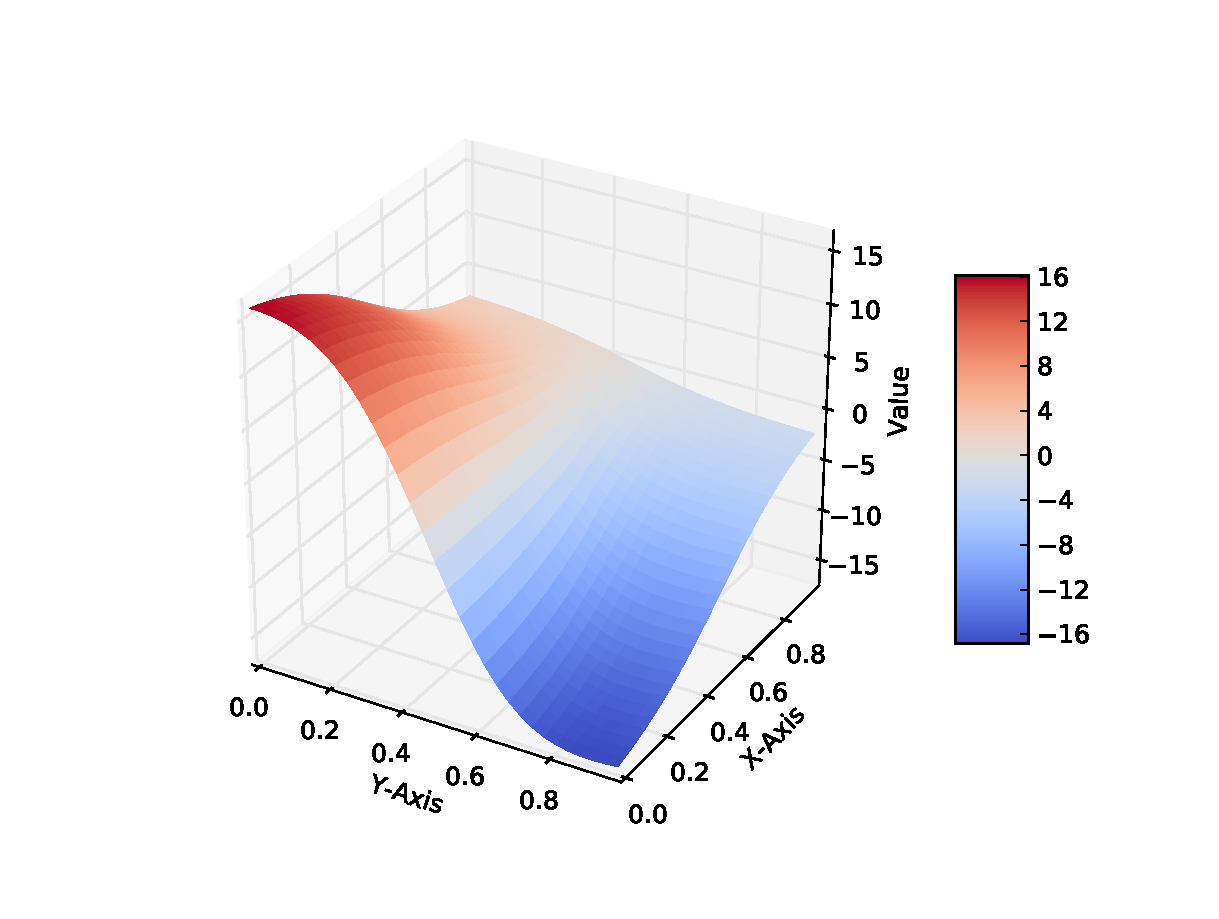
\includegraphics[width=\linewidth]{../writeup/figs/chap4/atan3s.pdf}
%  \endminipage
%  \minipage{0.12\textwidth}
%    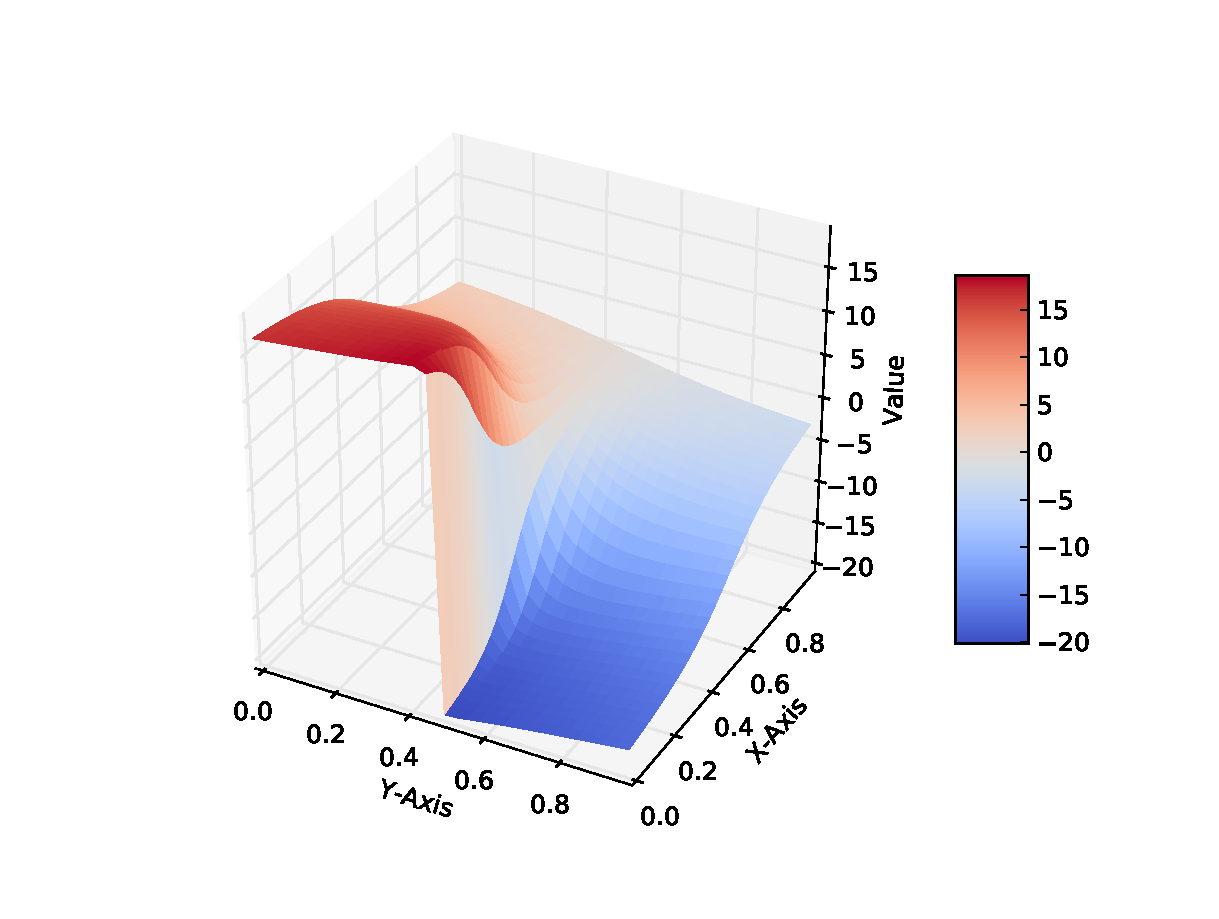
\includegraphics[width=\linewidth]{../writeup/figs/chap4/atan3e.pdf}
%  \endminipage
%  \minipage{0.12\textwidth}
%    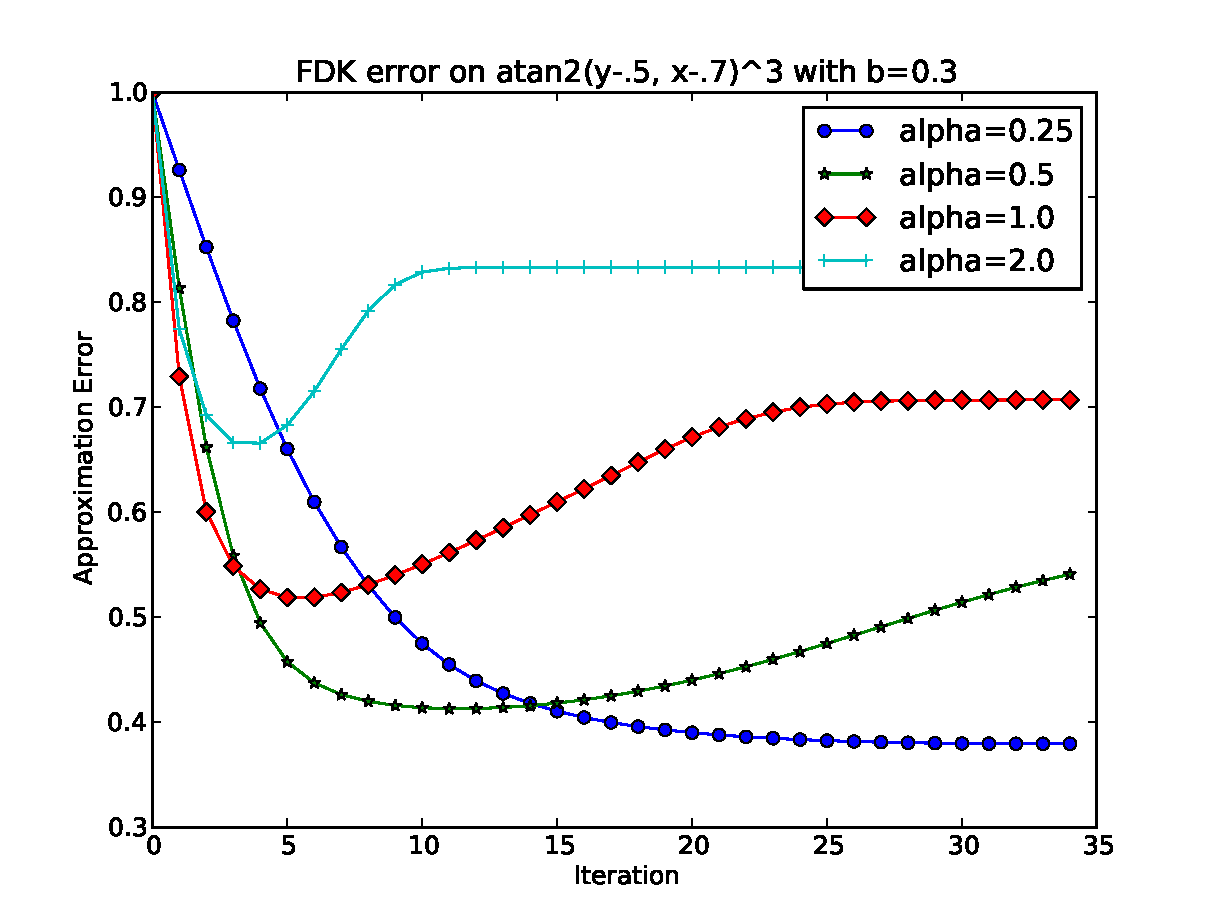
\includegraphics[width=\linewidth]{../writeup/figs/chap4/atanerr.pdf}
%  \endminipage
%\caption[Fitting the arctan]{Fitting $f(x,y) = \tan^{-1}(x - .7, y - .5)^3$.
%Left to right, the function being approximated, the kernel smoother fit, the best FDK fit,
%and the approximation errors over time.}
%\end{figure}
